% ! TeX root = ../../master-thesis.tex

\section{Step Simulation}
\label{section:design:step-simulation}

In order to address the halting problem, the previous simulation interface
should be refined to attain increased observability and controllability,
providing the user with more information about the state of the simulation. One
possibility is to model the concept of \textbf{step simulation}, which would
allow the user to execute a simulation step-by-step, receiving feedback after
every step (Figure \ref{figure:step-simulation}).

\begin{figure}[!ht]
  \centering
  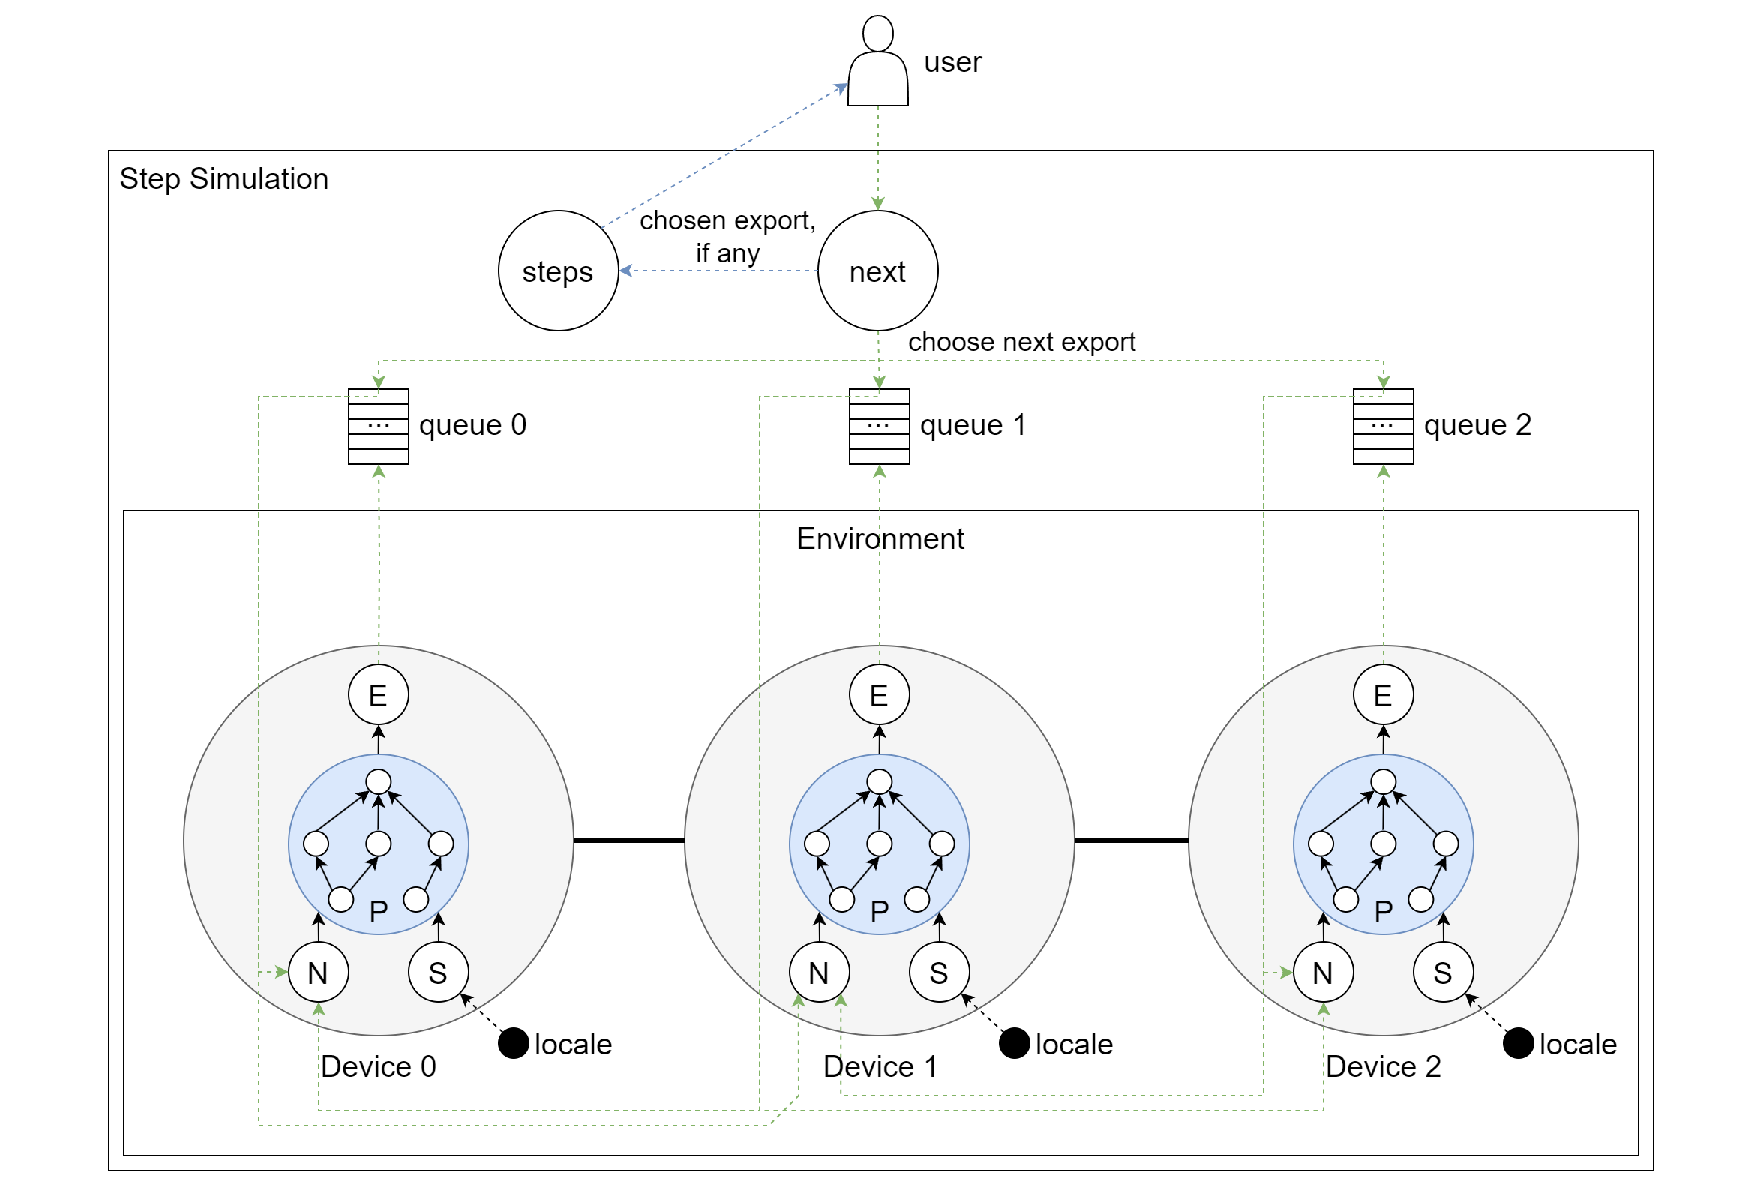
\includegraphics[width=1\textwidth]{resources/figures/step-simulation.pdf}
  \caption[The interface of a step simulation]{
    The interface of a step simulation. Each device owns a queue of exports
    that need to be transmitted. In fact, when an export is produced, it is
    inserted in the queue of the corresponding device, instead of being
    broadcast directly to its neighbors. The interface exposes new
    functionalities for selecting, transmitting (\texttt{next}) and observing
    (\texttt{steps}) the next export from the queues, increasing observability
    (the user can be notified if there are no more exports to be transmitted)
    and controllability (the user can decide exactly when the simulation should
    continue). The other functionalities of simulations are supported, but
    hidden for clarity.
  }
  \label{figure:step-simulation}
\end{figure}

The concept behind a step simulation involves keeping track of the exports of
the devices, deferring their propagation until requested by the user. This
strategy achieves greater observability since the simulation knows precisely
the number of pending exports, allowing the user to be notified when there is
none. Controllability is also increased, as the user can decide exactly when
the simulation should continue. Ultimately, the halting problem is solved if
the user has complete control over the environment. Indeed, in this scenario,
the user can reasonably assume that the evolution of the aggregate has
concluded (and the simulation should be stopped) when there are no more exports
to propagate and no further intention to change the environment.

In detail, the simulation maintains a queue of exports for each device, so that
the device exports are pushed into the queue of the corresponding device when
produced. The user can request the execution of the next \textbf{step} (i.e.,
the propagation of the next export), then an export is extracted from one of
the device queues and transmitted to the neighbors. For each request, the user
is notified of the extracted export or the lack of pending exports through the
reactive variable \texttt{steps}. Note how the system behaves exactly like the
base reactive model of FRASP if a request is sent as soon as a new export is
produced.

An added benefit of this approach is the ability to manage the scheduling of
device exports. When a user request is received, the simulation takes charge of
selecting the next export to transmit. To this end, various scheduling policies
can be implemented. For instance, the next export can be extracted from one of
the non-empty queues chosen randomly, ensuring non-determinism in the
aggregate's evolution. Alternatively, a round-robin policy can be employed to
select the next export, ensuring fairness in the simulation.

Concurrency is also supported as events from different export queues may be
propagated at the same time. However, synchronization is required to guarantee
a consistent view of the simulation from the perspective of the user.
